
\documentclass[../D+Manual.tex]{subfiles}
\begin{document}
\chapter{PDB (Atomic) Objects}

\begin{quote}
	My religion consists of a humble admiration of the illimitable superior spirit who reveals himself in the slight details we are able to perceive with our frail and feeble mind.\\
	\hspace*{\fill} \textit{Albert Einstein}
\end{quote}

Using an atomic description of a molecule gives a much higher resolution picture than using geometric models. For example, consider the tubulin hetero-dimer. It is comprised of an $\alpha$ and a $\beta$ dimer, both roughly spheres. However, the SAXS pattern of a pair of spheres is significantly different than that of the $\alpha\beta$ dimer. Using atomic representations can lead to much improved models, especially at higher resolutions (or higher $q$).


\section{PDB Files}

PDB files can be obtained from multiple sources. When downloaded from the \href{http://www.rcsb.org/pdb/home/home.do}{protein data bank}, the files usually work as-is. PDB files from simulations often disobey the \href{http://deposit.rcsb.org/adit/docs/pdb_atom_format.html#ATOM}{standard} and have various extensions.

A PDB file is a text representation of a collection atoms. From a certain point, atoms are represented like the following example:\\
\begin{lstlisting}[basicstyle=\tiny,breaklines=false,backgroundcolor=\color{gray!15},linewidth=1.07\linewidth]
         1         2         3         4         5         6         7         8
12345678901234567890123456789012345678901234567890123456789012345678901234567890
ATOM    145  N   VAL A  25      32.433  16.336  57.540  1.00 11.92      A1   N  
\end{lstlisting}

D+ requires that there be at least 78 characters per \texttt{ATOM} or \texttt{HETATM} (which stands for hetero (i.e. different) atom) line, as the atom type is determined by positions 77-78 (PDB v2.0 and greater)\footnote{If older versions are used or the line is less than 77 characters long, then D+ will attempt to determine the atom type from characters 13-14. No charge is assumed in this case. Note that \texttt{HG} will be interpreted as mercury and not as ``hydrogen-gamma'' even though that may be the intent coming out of GROMACS, for example. Other deviations from the standard
PDB file format should be amended (or removed from the file) before loading the file into D+.}. 
D+ reads and stores all the information, but the minimal information needed is shown here between the $\lfloor$ and $\rfloor$ symbols. Note that the spacing is critical.

\begin{lstlisting}[basicstyle=\tiny,escapeinside={(*}{*)},mathescape=true,backgroundcolor=\color{gray!15},linewidth=1.07\linewidth]
         1         2         3         4         5         6         7         8
12345678901234567890123456789012345678901234567890123456789012345678901234567890
ATOM    145  N   VAL A  25      32.433  16.336  57.540  1.00 11.92      A1   N1+
(*\hspace{-3pt} $\lfloor$ \hspace{3pt}*)   (* $\rfloor$ *)                       (*\hspace{-3pt} $\lfloor$ \hspace{3pt}*)     (* $\rfloor$ *)(*\hspace{-6.5pt} $\lfloor$ \hspace{3pt}*)     (* $\rfloor$ *)(*\hspace{-6.5pt} $\lfloor$ \hspace{3pt}*)     (* $\rfloor$ *)                     (*\hspace{-2pt} $\lfloor$ \hspace{0pt}*)(* $\rfloor$ *)
\end{lstlisting}


If there is a formal charge on the atom, it must appear in columns 79-80 of the line. A \texttt{HETATM} is processed exactly like an \texttt{ATOM}. Note that some simulations use various symbols to represent water molecules and these are not processed as such by D+. You will have to change the atom type to \ce{H} and \ce{O} manually.

MOLProbity \cite{ChenDz5180} can be used to add hydrogen atoms to PDB files. PyMOL \cite{PyMOL} can be used to add charges to residues that were supposed to be charged but the PDB file did not include the charges. The atomic form factor of ions, like O$^-$, differ from the form-factor of the corresponding neutral atom (O, in this example). D+ and take into account the atomic form factor of the 209 atoms and ions listed in the International Tables for Crystallography, using the five-Gaussian approximation \cite{hamilton1974international,marsh1983corrections}.    N$^+$, however, is not included in the International Tables for Crystallography and D+ computes the form factor of an N atom instead. If both  hydrogen atoms and charges are added to an N$^+$ group, an excess electron is obtained. An approximation that might be used to better account for an N$^+$ ion, is to manually remove from the PDB file, one of the hydrogen atoms next to the N$^+$ ion. This ensures that the correct total number of electrons in the protein is preserved. 


\section{PDB Objects in D+}

With high resolution data it is often useful to describe a protein structure as a collection of protein subunits.
The subunits can often be resolved using other methods (crystallography, simulations, etc.) and their results are usually available as PDB files.
One of the most important models D+ offers (accessible from the \hyperref[sec:domainView]{\texttt{Domain View}}) is that of a PDB file.
Once loaded, its parameters as shown in the \hyperref[sec:parameterEditor]{\texttt{Parameter Editor}} look like the following image.
\begin{figure}[h]
\centering
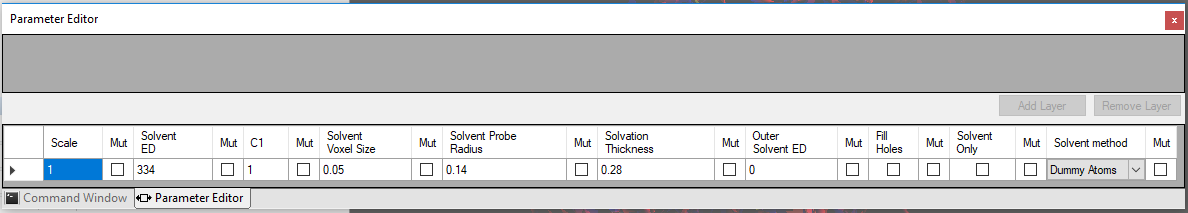
\includegraphics[width=1\linewidth]{PDBParameterEditor}
%\caption{}
\label{fig:PDBParameterEditor}
\end{figure}
\begin{wrapfigure}{r}{0.2\textwidth}
	\vspace{-20pt}
	\centering
	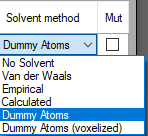
\includegraphics[width=1.1\linewidth]{PDBSolventMethods}
	\vspace{-30pt}
\end{wrapfigure}
Besides the \texttt{Scale} parameter, all the parameters relate to how the scattering amplitude of the solvent is subtracted from the atomic scattering amplitude.
When considering geometric shapes (cylinders, spheres, etc.), the electron density \textit{contrast} is trivial to obtain, as it is just the one shape minus a similar shape representing the solvent with a different electron density.
In the case of a collection of atoms, treating the solvent is not so trivial.
D+ offers two main methods to subtract the solvent contribution, and account for the contribution of the solvation layer:
\begin{equation}\label{sv}
F(\vec{q})=a\cdot F^v_{\text{mol}}(\vec{q}) - \rho_{0}\cdot f_{\text{Excluded Solvent}}^{\text{Dummy Atom}}(\vec{q}) + \left(\rho_{\text{Solvation Layer}}-\rho_{0}\right) \cdot F_\text{Solvation Layer}\left(\vec{q}\right)
\end{equation}
that uses \texttt{Dummy Atoms} Gaussian spheres to account for the excluded volume of atoms. Alternatively, the excluded volume can be taken into account as a collection of voxels:    
\begin{equation}
\label{sv2}
F(\vec{q})=a\cdot F^v_{\text{mol}}(\vec{q}) - \rho_{0}\cdot F^{\text{Voxel}}_\text{Excluded Solvent}(\vec{q}) + \left(\rho_{\text{Solvation Layer}}-\rho_{0}\right) \cdot F_\text{Solvation Layer}\left(\vec{q}\right)
\end{equation}
$F^v_{\text{mol}}$ is explained in Equation \ref{eq:FvMol}, $f_{\text{Excluded Solvent}}^{\text{Dummy Atom}}$ in Equation \ref{eq:ExcludedDummy},
$F^{\text{Voxel}}_\text{Excluded Solvent}$ in Equation \ref{eq:ExcludedVoxels}, and $F_\text{Solvation Layer}$ in Equation \ref{solvation}.

$a$ is equal to $1$, unless \texttt{Solvent Only} is indicated in the \texttt{Parameter Editor} of D+, in which case $a=0$.
If $a$ is set to $0$ and, in addition, \texttt{Solvent ED} (the mean solvent electron density, $\rho_{0}$), is set to 0, we get the contribution to the scattering amplitude only from the solvation shell.
By loading a PDB and computing equation \ref{sv} using a finite value for the \texttt{Outer Solvent ED} (the solvation layer electron density, $\rho_{\text{Solvation Layer}}$),  and \texttt{Solvent ED} (or $\rho_{0}$), in units of $\SI{}{\elementarycharge\cdot\nm^{-\cubed}}$, the solvent contribution to the scattering is computed based on the radii taken from \cite{fraser1978improved,slater1964atomic,svergun1995crysol}.
The excluded volume and solvation shell are then calculated based on the chosen radii.

If \texttt{Outer Solvent ED}, $\left(\rho_{\text{Solvation Layer}}\right)$, is set to $0$, when a PDB file is loaded, D+ does not add any solvation layer. If the same PDB is reloaded and only the contribution from the solvation shell is computed [by indicating \texttt{Solvent Only} (i.e. $a=0$), and by setting  \texttt{Solvent ED},  $\rho_{0}$, to 0,  and \texttt{Outer Solvent ED},  $\rho_{\text{Solvation Layer}}$, to  $\rho_{\text{Solvation Layer}}-\rho_{0}$], any other method for calculating the solvation shell can be applied and its contribution can be added to the contributions of the vacuum term (i.e \texttt{Outer Solvent ED}=0, and \texttt{Solvent ED} = 0) and the \texttt{Dummy Atoms} term. Splitting the computation in this mode has another advantage. Fitting the value of the solvation layer contrast, $\rho_{\text{Solvation Layer}}-\rho_{0}$, becomes faster, as it is equivalent to setting \texttt{Ourter Solvent ED}=1 (or $\rho_{\text{Solvation Layer}}=1$) and fitting the \texttt{Scale} factor of the solvation shell amplitude, and hence does not require to compute a new grid for the voxels of the solvation shells.  

\subsection{Gaussian ``Dummy'' Atoms}

To account for the excluded volume of the atoms, it has been suggested to subtract a Gaussian sphere from each atom, where the center of the sphere is located at the atom coordinate  \textcite{fraser1978improved}. Therefore, D+ subtracts the Fourier transform of the following normalized Gaussian sphere:
\begin{equation*}
	F^d_j\left(q\right) =
	\rho_{0}\cdot V_j \cdot\exp
	\left[-\frac{V_m^{2/3}\cdot q^2}{4\pi}\right],
\end{equation*}
where $V_j=\frac{4\pi}{3}r^3_j$ is the volume of atom $j$, and $V_m = \sum_{j} V_j$ is the mean atomic volume over the entire molecule. $r_j$ is an effective atomic radius (dictated by the type of atom) and $\rho_{0}$ is the mean solvent electron density (\texttt{Solvent ED}). D+ accepts both positive and negative values of $\rho_{0}$. Negative $\rho_{0}$ values are nonphysical, however, they might be useful in special cases. D+ always \textbf{subtracts} the excluded volume amplitude, $F_j^d$, from other amplitudes (see Equation \ref{eq:fmF}). Negative $\rho_{0}$ can be used to \textbf{add} the contribution of $F_j^d$ to other amplitudes. Caution should be taken, if solvation layer is added, as a negative $\rho_0$ value will also impact Equations \ref{sv}, \ref{sv2}, \ref{ExcludedSolvent}, and \ref{eq:SolvatedMolecule}.
The scattering amplitude from atom $j$ after subtracting the contribution of the solvent is:
\begin{equation}
f^\circ_j\left( q \right) -F_j^d\left( q \right) 
\label{eq:fmF}
\end{equation}
where $f^\circ_j\left( q \right)$ is the scattering amplitude of the $j$-th atom \textit{in vacuo} (using the five Gaussian approximation):
\begin{equation}\label{FiveGaussinan}
f_{i}^{0}\left(q\right)=\sum_{k=1}^{4}a_{k}\cdot \exp{\left(-b_{k}\left(\frac{\left|\vec{q}\right|}{4\pi}\right)^{2}\right)}+c.
\end{equation}
The coefficients $a_{k},b_{k}$, and $c$ are the Cromer-Mann coefficients, given in units of the Thomson scattering length, $r_0$. Note that in D+, however, $r_0$ is set to $1$.

The solvent contribution can be modulated like
\begin{equation*}
f_{j}^{s}(q)=f^\circ_j\left( q \right) - C_1\left(q\right) F^d_j\left( q \right) 
\end{equation*}
where

\begin{equation*}
C_1\left(q\right) = c^3_1\cdot\exp
	\left[-\frac{V_m^{2/3}\cdot q^2\left(c_1^2 -1\right)}{4\pi}\right].
	\label{c1}
\end{equation*}
is used to uniformly adjust $V_m$ and $c_1$ is a scaling factor \parencite{schneidman2013accurate}.
The default value for $c_1$ is 1 (making it not affect the solvent subtraction) and the default constraints are $\left[0.95,1.05\right]$.
This method is coined \texttt{Dummy Atoms} in the drop down menu above.

The solution scattering amplitude from a molecule, given by a list of $n$ atoms, whose coordinates are $\vec{r}_j$, is:
\begin{equation*}
F^s_{\text{mol}}\left(\vec{q}\right)=\sum_{j=1}^n f_{j}^{s}(q)\cdot \exp\left(i\vec{q}\vec{r}_j\right).
\end{equation*}


\noindent If \texttt{Solvent ED} or $\rho_{0} = 0$, we get the scattering amplitude of the molecule in vacuum:
\begin{equation}
F^v_{\text{mol}}\left(\vec{q}\right)=\sum_{j=1}^n f_{j}^{0}(q)\cdot \exp\left({i\vec{q}\vec{r_{j}}}\right).
\label{eq:FvMol}
\end{equation}

\noindent The contribution of the excluded volume to the amplitude is
\begin{equation}
\rho_{0}\cdot f_{\text{Excluded Solvent}}^{\text{Dummy Atom}}= C_1\left(q\right)\cdot
\sum_{j=1}^n F^d_{j}(q)\cdot \exp\left(i\vec{q}\vec{r}_j\right)
\label{eq:ExcludedDummy}
\end{equation}

\noindent All the other options for solvent subtraction pertain to the following method.

\subsection{Voxel Based Solvent}
\label{sec:Voxel}
An alternative solvent subtraction method is to determine the shape that is the union of all the atoms and subtract that (at the electron density of the solvent).
This was proposed by \textcite{Pavlov}.
This methods makes a few assumptions and has some shortcomings.

The solvent excluded volume is calculated in several stages.
First of all, space is discretized into voxels of a specific size, determined by the \texttt{Solvent Voxel Size} parameter, given in $\unit{nm}$ and its default value is $\unit[0.2]{nm}$.
Each voxel is marked as occupied if at least one atom's coordinate is within that atom's radius (the atomic radius type can be chosen in the \texttt{Solvent method} parameter, including the radii of the Gaussian dummy atoms, given in \texttt{Dummy Atoms (voxelized)}).
This represents the excluded volume of the atomic structure.

The contribution of the excluded solvent to the scattering amplitude is computed as the sum over the scattering amplitudes from the collection of voxels (or boxes) comprising the solvent excluded volume. 
The scattering amplitude of the $j$th voxel (or box) of dimensions, $\omega_j,\tau_j$, and $\mu_j$,  whose center is at $\vec{r}_j^{\text{Voxel}}$ is (see \textcite{szekely2010solution}):

\begin{equation}
f_j^{\text{Voxel}}\left(\vec{q}\right) = \frac{8}{q_x \cdot q_y \cdot q_z}\sin\left(\frac{q_x \omega_j}{2}\right)\sin\left(\frac{q_y \tau_j}{2}\right)\sin\left(\frac{q_z \mu_j}{2}\right)
\cdot 
\exp\left(i\cdot \vec{q}\cdot\vec{r}_j^{\text{Voxel}}\right) 
\end{equation}

\noindent The total scattering amplitude of the excluded voxels is then a sum over the solvent excluded voxels:
\begin{equation}
F^{\text{Voxel}}_\text{Excluded Solvent}\left(\vec{q}\right) = \sum_{j\in\{\text{Excluded Voxels}\}} f_j^{\text{Voxel}}\left(\vec{q}\right)
\label{eq:ExcludedVoxels}
\end{equation}
and the scattering amplitude of the molecule in the solution is:
\begin{equation}
F^s_{\text{mol}}\left(\vec{q}\right)=F^v_{\text{mol}}\left(\vec{q}\right) -\rho_{0}\cdot F^{\text{Voxel}}_\text{Excluded Solvent}\left(\vec{q}\right).
\label{ExcludedSolvent}
\end{equation}

\subsection{Solvation Layer}
To obtain the contribution of a solvation layer around an atomic structure, the solvent excluded volume is determined, as explain in \ref{sec:Voxel}, using the selected \texttt{Solvent method}.  
A probe with a radius of \texttt{Solvent Probe Radius} (in \unit{nm}) determines the accessible surface of the protein. The default value of the probe radius is $\SI{0.14}{\nm}$, which corresponds to the radius of a water molecule.
All voxels that are within \texttt{Solvation Thickness} (in \unit{nm}) of the surface and are not occupied by an atom are marked as occupied by a solvation layer, and their mean electron density (ED), $\rho_{\text{Solvent Layer}}$, is given by the value of \texttt{Outer Solvent ED} (in units of $\SI{}{\elementarycharge\cdot\nm^{-\cubed}}$). If \texttt{Outer Solvent ED} = 0, D+ ignores the contribution from the solvation layer.
Voxels that are completely enveloped by the union of the two shapes are considered holes.
If the \texttt{Fill Holes} checkbox is checked, these voxels will be added to the shape that represents the volume of the atoms (as excluded volume).
The excluded volume shape with an electron density of \texttt{Solvent ED}, $\rho_{0}$ (in units of $\SI{}{\elementarycharge\cdot\nm^{-\cubed}}$), is subtracted from the atomic contributions (Equation \ref{ExcludedSolvent}).
The solvation layer represents the electron density contrast owing to a higher or lower density of the solvent near the surface of the atomic structure, with respect to the bulk solvent. 

The contribution of the solvation layer to the scattering amplitude is computed as the sum over the scattering amplitudes from the collection of voxels comprising the solvation layer. 
The amplitude of the solvation layer is then:
\begin{equation}
F_\text{Solvation Layer}\left(\vec{q}\right) = \sum_{j\in\{\text{Solvation Layer Voxels}\}} f_j^{\text{Voxel}}\left(\vec{q}\right).
\label{solvation}
\end{equation}
The scattering amplitude of the solvated molecule is:
\begin{equation}
F_\text{Solvated Molecule}\left(\vec{q}\right) = F^s_{\text{mol}}\left(\vec{q}\right) + \left(\rho_{\text{Solvation Layer}}-\rho_{0}\right) \cdot F_\text{Solvation Layer}\left(\vec{q}\right).
\label{eq:SolvatedMolecule}
\end{equation} 
 



%TODO explain how to use Dplus to subtract dummy atoms and to add solvation layer (using one or two different models). 
Computations of voxel based excluded volume and solvation layer can take a significant amount of time, particularly when using CPU. Fitting the parameters should therefore be done manually rather than by the fitting algorithms of D+. In \S9 % check reference
of the Supporting Online Materials (SOM) of the paper about D+ \cite{Dplus2017} there are several examples that demonstrate how to compute the solvation layer of large complexes, containing many subunits, in a scalable manner. 

\subsection{Implicit/Explicit Hydrogen Atoms}
\label{sec:implicitExplicit}

Hydrogen atoms are often not listed in PDB files that originate in protein and/or nucleic acid crystallography.
On the flip side, they are usually included in files originating from simulations, or can be added to the PDB file by software like \textit{MolProbity} (see \cite{ChenDz5180}).
Furthermore, their scattering contribution is not negligible in proteins and/or nucleic acids.
To accurately take the hydrogen atoms into account when they are missing from the PDB file, each amino acid or nucleic base is looked at (based on the number at positions 23-26 in the PDB file).
If there is at least one hydrogen atom within the amino acid residue or nucleic  base, then nothing is changed.
If there are no hydrogen atoms, then the collection of lines is further examined.
If all the atoms correspond to atoms within the specific amino acid or nucleic base (based on characters 13-16, \textit{e.g.} \texttt{CG2}, or carbon-gamma number 2) then the different atoms within the amino acids or nucleic bases are modified so that their relevant hydrogen atoms' contributions are added to the heavier atoms they are bonded to.
If the amino acid or nucleic base name (characters 23-26) is not recognized, there is at least one explicit hydrogen atom in the amino acid or nucleic base, or if there is an unidentified atom (characters 18-20) then only the explicitly listed hydrogens are taken into account.
Otherwise, they will be taken into account implicitly.

The implicit addition of H atoms modifies the five Gaussian approximation for the heavier atom (see Table 1 in \cite{Dplus2017}).
The implicit hydrogen atoms change the heavier atoms' effective radii as in Table 1 in \textcite{svergun1995crysol}.
This affects the subtracted solvent and the radii used for the solvation layer.
\section{PDB files of structures with repeating subunits}
If a large PDB file contains repeating subunits, the computation can be done faster, using \hyperref[PDBUnit]{\texttt{PDBUnits}}, which finds all the instances
of the subunit within a large structure. The tool
exports the \hyperref[chp:Symmetries]{\texttt{Assembly Symmetry}} of the subunit as a docking list (DOL) text file, which can then be used by D+ together with the PDB of the subunit to compute the contribution of all its instances to the scattering amplitude. 

\section{Anomalous Scattering} \label{sec:anomalousScattering}
D+ can take anomalous scattering of atoms into account when computing scattering amplitudes of atomic models. Two additional correction terms should be added to get the atomic form factor energy dependence:
\begin{equation*}
	f(q,\lambda) = f^\circ(q) + f'(\lambda) + i f''(\lambda).
\end{equation*}

When selecting a \texttt{PDB File...} in the the dropdown menu in  \hyperref[sec:domainView]{\texttt{Domain View}} window, the \texttt{Anomalous} checkbox will appear. Selecting the checkbox will cause a file selection window to launch, and you can choose an \texttt{Anomalous file}. Unselecting the checkbox will cause the \texttt{Anomalous File} to be removed.
Select the text file containing the relevant $f'$ and $f''$ values.
The file should be formated using any combination of the lines below.

\lstset{style=anomalousFile,}

\begin{lstlisting}
# Energy    2345.82km
# <f'>  <f''>   <atom identifier>
1.2     2.3     Fe2+
#<f'>   <f''>   <atom indices>
1.3     3.4     125     256
#<f'>   <f''>   <name of a group that's defined below>
-3e4    +2.01   $(someRandomGroupName)
#<name of a group>      <list of atom indices>
$(someRandomGroupName)  252 472 7344 313
\end{lstlisting}

Lines that start with '\#' are considered comments and are ignored.
%TODO add an example. What do you mean by atom indices (line in the pdb file?) and group name (CH, CH_2?)? 
The \texttt{Example Files} subfolder of D+ includes more examples. 

Please note: only \textbf{Monte Carlo} integration method can be used for anomalous scattering. 


\section{DebyeCalculator}


\texttt{DebyeCalculator} is a command line executable program that is located at \path{C:\Program Files\D+\bin>} or where ever D+ was installed.
 
In this folder, typing \texttt{DebyeCalculator.exe -h} will print the help menu of the program, which provides the allowed options:

\texttt{-h [ --help ] arg} 

Print this help message

\texttt{-i [ --PDBFile ] arg}

Input PDB file

\texttt{-o [ --out ] arg (=Debye.out)}

The name of the file to write the results to

\texttt{-g [ --gpu ] [=arg(=1)] (=0)}

Use a GPU to calculate if available

\texttt{-p [ --progress ] [=arg(=1)] (=1)}

Print progressbar

\texttt{-s [ --sol ] [=arg(=333)]} 

The solvent electron density to be subtracted as Gaussians

\texttt{-c [ --c1 ] arg (=1)}

The c1 value used to adjust the excluded volume of the atoms

\texttt{-d [ --deb ] [=arg(=1)] (=0)} 

Take the B factor into account if available

\texttt{--qMin arg (=0)}

The minimum q value from which the intensity will be calculated

\texttt{-q [ --qMax ] arg (=6)}

The maximum q value to which the intensity will be calculated

\texttt{-n [ --qVals ] arg (=512)}

The number of points to be calculated

\texttt{-k [ --kernel ] arg (=2)}

The version of the GPU kernel to use. Not
safe. Don't assume any number works unless
you know what you're doing. Valid options:
are \texttt{1,2}, or \texttt{4}. Other values will fail.

\subsection{Examples}

The simplest usage example would be:

\path{C:\Program Files\D+\bin>DebyeCalculator.exe -i C:\Users\owner\Downloads\1jff.pdb -o C:\Users\owner\Downloads\1jffDebye.out}

\noindent The same results will be obtain by: 

\path{C:\Program Files\D+\bin>DebyeCalculator.exe -i C:\Users\owner\Downloads\1jff.pdb -o C:\Users\owner\Downloads\1jffDebyeS.out -g 0 -p 1 -s 333 -c 1 -d 0 0 -q 6 -n 512}


\printbibliography[heading=subbibliography]
\end{document}